\begin{frame}
    \titlepage
\end{frame}



\begin{frame}
    \frametitle{Introduzione  alle Botnet}
    \begin{definition}[Botnet]
        Rete di host compromessi chiamati bot, che eseguono istruzioni impartite da host detto botmaster, attraverso l'ausilio di un server che funge da tramite,  detto Command And Control Server (C\&C).
    \end{definition}
    Definita da:
    \begin{itemize}
        \item Topologia
              \begin{itemize}
                  \item Centralizzata
                  \item Decentralizzata (P2P)
                  \item Ibrida
              \end{itemize}
        \item Schema comunicazionale:
              \begin{itemize}
                  \item propagazione
                        \begin{itemize}
                            \item attiva
                            \item passiva
                        \end{itemize}
                  \item operazione
              \end{itemize}
        \item Protocolli utilizzati
        \item Tecniche di occultamento/offuscamento
    \end{itemize}
\end{frame}

\begin{frame}
    \frametitle{Realizzazione dell'infrastruttura di testing}
    \begin{columns}
        \begin{column}{0.5\textwidth}
            Principali tecnologie analizzate:
            \begin{itemize}
                \item Server VMWare ESXi
                \item Firewall
                      \begin{itemize}
                          \item Netfilter
                          \item Iptables
                          \item NFtables
                          \item Firewalld
                      \end{itemize}
                \item Docker
            \end{itemize}
        \end{column}
        \begin{column}{0.5\textwidth}
            \begin{figure}
                \centering
                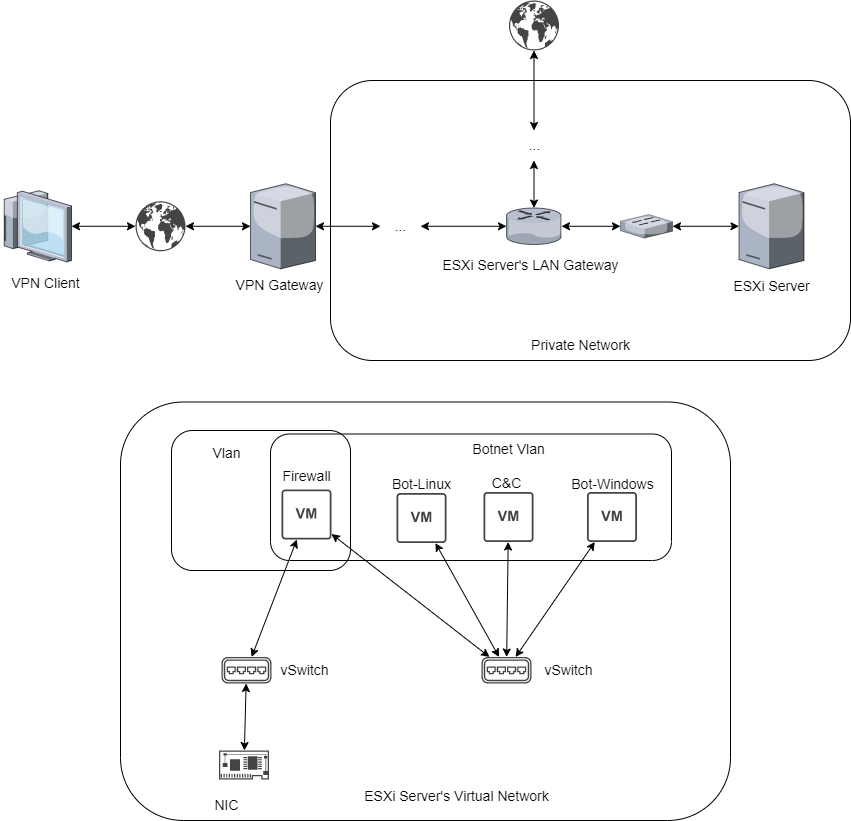
\includegraphics[width=\textwidth]{res/fig/infrastruttura1.png}
            \end{figure}
        \end{column}
    \end{columns}
\end{frame}

\begin{frame}
    \frametitle{Intrusion Detection System (IDS)}
    \begin{columns}
        \begin{column}{0.5\textwidth}
            Categorizzabili in:
            \begin{itemize}
                \item Signature based (SIDS)
                \item Anomaly based (AIDS)
            \end{itemize}
            In particolare sono stati approfonditi ed utilizzati:
            \begin{itemize}
                \item Security Onion
                \item Ossim
            \end{itemize}
            Utilizzati principalmente come NIDS.
        \end{column}
        \begin{column}{0.5\textwidth}
            \begin{figure}
                \centering
                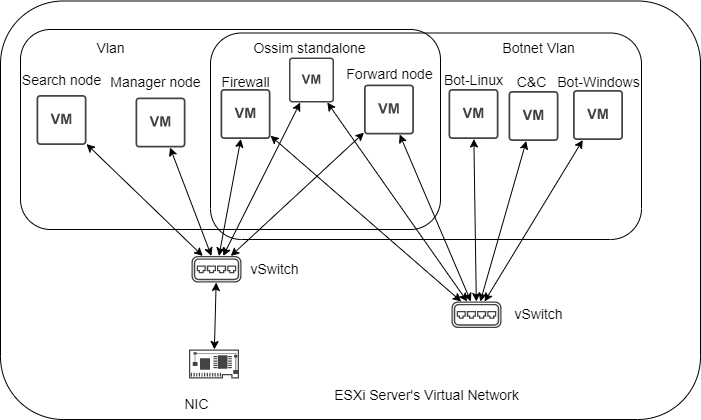
\includegraphics[width=\textwidth]{res/fig/infrastruttura2.png}
            \end{figure}
        \end{column}
    \end{columns}
\end{frame}